2;rgb:0000/0000/0000\chapter{Reading and Writing Images}
\label{sec:IO}

This chapter describes the toolkit architecture supporting reading and
writing of images to files. OTB does not enforce any particular file
format, instead, it provides a structure inherited from ITK,
supporting a variety of formats that can be easily extended by the
user as new formats become available.

We begin the chapter with some simple examples of file I/O.

\section{Basic Example}
\label{sec:ImagReadWrite}
\input{ImageReadWrite.tex}

To better understand the IO architecture, please refer to Figures
\ref{fig:ImageIOCollaborationDiagram},
\ref{fig:ImageIOFactoriesUseCases}, and
\ref{fig:ImageIOFactoriesClassDiagram}.

\begin{figure}
\center
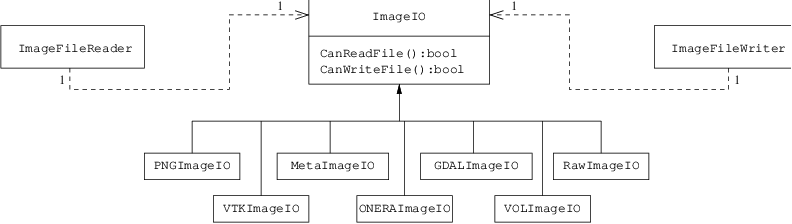
\includegraphics[width=\textwidth]{ImageIOCollaborationDiagram.eps}
\itkcaption[Collaboration diagram of the ImageIO classes]{Collaboration diagram
of the ImageIO classes.} \label{fig:ImageIOCollaborationDiagram}
\end{figure}

\begin{figure}
\center
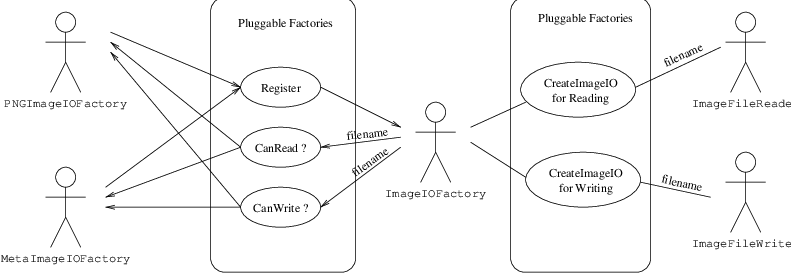
\includegraphics[width=\textwidth]{ImageIOFactoriesUseCases.eps}
\itkcaption[Use cases of ImageIO factories] {Use cases of ImageIO factories.}
\label{fig:ImageIOFactoriesUseCases}
\end{figure}

\begin{figure}
\center
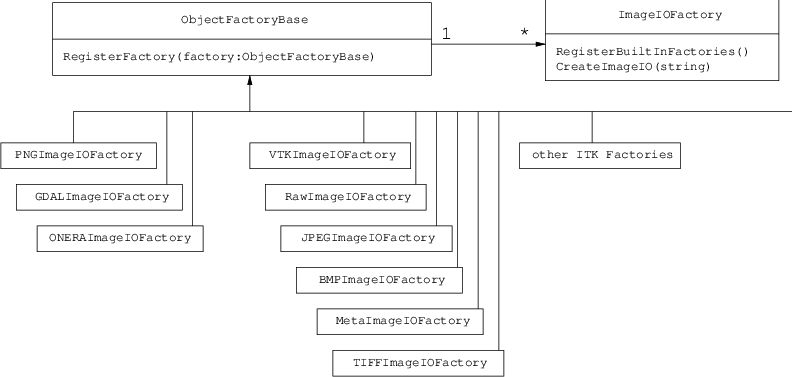
\includegraphics[width=\textwidth]{ImageIOFactoriesClassDiagram.eps}
\itkcaption[Class diagram of ImageIO factories] {Class diagram of the ImageIO
factories.}
\label{fig:ImageIOFactoriesClassDiagram}
\end{figure}


The following section describes the internals of the IO architecture provided
in the toolbox.

\section{Reading, Casting and Writing Images}
\label{sec:ImagReadCastWrite}
\input{ImageReadCastWrite.tex}

\section{Extracting Regions}
\label{sec:ImagReadRegionOfInterestWrite}
\input{ImageReadRegionOfInterestWrite.tex}


\section{Reading and Writing Vector Images}
\index{Image!Multispectral}
\label{sec:VectorImagReadWrite}

Images whose pixel type is a Vector, a CovariantVector, an Array, or a Complex
are quite common in image processing. One of the uses of these tye of
images is the processing of SLC SAR images, which are complex.


\subsection{Reading and Writing Complex Images}
\label{sec:ComplexImagReadWrite}
\input{ComplexImageReadWrite.tex}

\section{Reading and Writing Multiband Images}
\label{sec:MultibandImagReadWrite}
\input{MultibandImageReadWrite.tex}

\subsection{Extracting ROIs}
\label{sec:ExtractROI}
\input{ExtractROI.tex}

\section{Reading Image Series}
\label{sec:ReadingImageSeries}
\input{ImageSeriesIOExample}

